\documentclass[a4paper]{article}
\usepackage[left=3cm, right=3cm]{geometry}
\usepackage{hyperref}
\usepackage{cite}
\usepackage{amssymb}
\usepackage{url}
\usepackage{float}
\usepackage{longtable}
\usepackage{array}
\usepackage{algorithmic}
\usepackage[boxed]{algorithm}
\usepackage{color}
\usepackage{graphicx}
\usepackage{tabularx}
\usepackage{caption,subcaption}
\pagestyle{headings}
\newcommand{\secondo}{\textsc{Secondo}}
\newcommand{\bmodb} {BerlinMOD Benchmark}
\newcommand{\op}[1]{\textbf{#1}}
\newcommand{\dt}[1]{\textsl{\underline{#1}}}
\newcommand{\true}{\textsl{TRUE}}
\newcommand{\false}{\textsl{FALSE}}
\newcommand{\secver}{2.9.StableNewFlob}
%opening
\title{Network Data Model and BerlinMOD Benchmark}
\author{Simone Jandt}
\date{Last Update: \today}
\begin{document}
\maketitle
\begin{abstract}
In the past several data models for the representation of spatio-temporal data
objects have been developed. Among others we can categorize this data models
into data models for objects moving freely in the two dimensional space and data
models for network constrained moving objects. In the mean time two representants
of this data models, one for each category, have been implemented in
\secondo{} DBMS. We used the \bmodb{} to compare the capabilities of the both
data models. The results are shown in this paper.

The very good results of the network data model in this comparsion encourages us
to propose a extension of the \bmodb{} with a additional query set BerlinMOD/Net.
This new query set covers the specialised challenges for network constrained
data models and enables us to use the \bmodb{} to compare the capabilities of
different network data models with respect to this specialised network challenges.
\end{abstract}
\section{Introduction}
In the past several data models for the representation of spatial and
spatio-temporal data objects have been developed. Among others we can categorize
them into data models for objects moving freely in (two dimensional) space and
data models for network constrained moving objects. For both categories
several different data models have been presented like
\cite{335426,chenzaniolosqlst} for spatio-temporal data objects moving freely in
 space and \cite{1146465,956692,VazWolfNetMod} for spatio-temporal data objects
that are constrained by given networks to name just a few.

For our experiments we choosed one example data model as representative for
each of the both categories to compare the capabilities of the both different
data models. Spatio-temporal objects moving freely in two dimensional space are
represented by the data model presented in \cite{335426}. And network constrained
data models are represented by the network data model presented in \cite{1146465}.
Both data models are available in the \secondo{} DBMS and use the same temporal representation. So we can exclude that the use of different DBMS or temporal
representations bias the results of our comparision.

As we use \secondo{} it seems to be a logical next step to use the \bmodb{} \cite{BerlinMODVLDB} to compare the capabilities of the
both data models. The \bmodb{} is best to our knowledge the first benchmark for
complete spatio-temporal database systems and it is also available in the \secondo{}
 DBMS. Furthermore the \bmodb{} data model is the data model of freely movement
in two dimensional space that we use for our comparison. So we only have to
transform the \bmodb{} spatial and spatio-temporal data types once into our
network data model representation. This avoids sources of errors and makes the
correctness controll of the query results more easy.

In our experiments the network data model outperforms the data model of free
movement in space significantly. The total run time for all benchmark queries
is less than half as long for the network model as the total run time for
the data model of free movement in the space. Such that it seems useful to
develope specialised databases and operations for network constrained moving
objects. In the same way the storage space used for the trips in the network
data model is less than 60\% of the storage space used by the data model of free
movement in the space. Also the number of units in the network data model is
less than 50\% of the number of units in the data model of free movement in the
space.

The very good results of the network data model encourages us to propose the extension
of the \bmodb{} by a query set BerlinMOD/Net. The new query set covers the specialised
challenges of network data models like network distance computing which are not
covered by the original \bmodb{}. The new query set should enable us to compare
the capabilities of different network data models with respect to the special
challenges of network constrained data models.

The rest of the paper is organised as follows: In section \ref{sec:relWork} we give a
short reminder of the underlying \secondo{} DBMS (\ref{sec:secondo}), the \bmodb{} (\ref{sec:bmodb}) and the two data models (\ref{sec:bmodbdatamod}
 and \ref{sec:netdatamod}) we choosed as representatives for our comparision.
In section \ref{sec:bmodbNetDataMod} we present the setup for our experiments (\ref{sec:scenario}) and describe our transformation of the \bmodb{} data and
queries in the network data model representation (\ref{sec:Translation}). The
results of our experiments are presented in section (\ref{sec:results}). At least
we present our proposed extension of the \bmodb{} for network data models in section \ref{sec:newqueries} and conclude our work in section \ref{sec:summary}.
\section{Related Work}
\label{sec:relWork}
As mentioned before in the past other data models for free movement in the space \cite{335426,chenzaniolosqlst} and for network constrained movement have been
presented \cite{1146465,956692,VazWolfNetMod}. As well there are some more
benchmarks \cite{COSTBenchmark, QueriesTheodoridis} and database systems for
spatial and spatio-temporal datatypes \cite{HERMES,1054151}. But they don't
provide a combination of different implemented and supported data types together
 with a existing benchmark like the actual \secondo{} DBMS. So it is self-evident
for us to use the \secondo{} DBMS in combination with the provided data types and
the \bmodb{} to compare the capabilities of the both different data models.

In the next subsections we give short reminders of the \secondo{} database system (\ref{sec:secondo}), the \bmodb{} (\ref{sec:bmodb}), and the both data models (\ref{sec:bmodbdatamod}, \ref{sec:netdatamod}) we used in our experiments.
\subsection{Secondo}
\label{sec:secondo}
The extensible \secondo{} DBMS presented in \cite{686903,1054151} provides a
platform for implementing various kinds of data models. It provides a clean
interface between the data model independent system frame and the content of the
 single data models. Hence \secondo{} can be easily extended by the user
implementing so called \secondo{} algebra modules to introduce  new data types
and operations on this data types. The user also may define additional viewers
for the graphical user interface or write optimization rules or cost functions
to extend the optimizer. \secondo{} is free available in the web \cite{secondoweb}
and comes with a number of already implemented spatial and spatio-temporal data types
and operations including the spatio-temporal data model of free movement in the space \ref{sec:bmodbdatamod} and the network data model \ref{sec:netdatamod}. Furthermore the \bmodb{} descripted in \ref{sec:bmodb} has been developed in the \secondo{} DBMS.
For our experiments we used the \secondo{} version \secver{}.
\subsection{BerlinMOD Benchmark}
\label{sec:bmodb}
The \bmodb{} was presented in \cite{BerlinMODVLDB} \nocite{BerlinMOD} and the
provided scripts for the data generator are implemented as \secondo{} DBMS operations.
The \bmodb{} is available in the web \cite{berlinmodweb} and provides a well defined
data-set and queries for the experimental evaluation of different moving object
data representations. The \bmodb{} emphasises the development of complete systems
and simplifies experimental repeatability pointing out the weakness and the potency
of the benchmarked systems.

The data-sets of the \bmodb{} are created using the street map of the German
captial Berlin \cite{bbike} and statistical data about the regions of Berlin
\cite{bevberlin,berlinstadtatlas} as input relations.
The created moving objects represent cars driving in the streets of Berlin,
simulating the behaviour of people living and working in Berlin.
Every moving object has a home node and a work node. Every weekday each car will
do a trip from the home node to work the work node in the morning and vice versa
in the late afternoon. Besides this randomly choosen cars will make additional
trips in the evening and up to six times at the weekend to randomly choosen
targets in Berlin. Because for all this the street network of Berlin is used to
generate the moving object data sets the \bmodb{} can also be used to benchmark
network constrained moving object data models.

The number of observed cars and the duration of the observation period can be
influenced setting the $SCALEFACTOR$ to different values in the data generation
script of the \bmodb{}. For example at $SCALEFACTOR$ 1.0 the data generator
creates 2000 moving objects observed for 28 days. Each of them sending a
GPS-signal every 2 seconds. This simulated signals are simplified such that time
intervals when a car doesn't move or moves in the same direction at the same
speed are merged into one moving unit. This means that if for example a car parks
8 hours in front of the work node there will be only one entry in the cars history of movement with a time interval of 8 hours instead of 14.400 entries one for each
GPS interval.

The \bmodb{} provides two different approaches to store the histories of moving
objects. On the one hand the object-based approach (OBA) and on the other hand
the trip based approach (TBA).

In the OBA the complete history for each moving object
is kept together into one single entry. There is only one relation (dataScar)
containing one tuple for each object consisting of the spatio-temporal data of
the object (journey), the licence, the type, and the model of the object.

In the TBA we have two relations. One of them (dataMcar) contains the static data
for each object like licence, type, and model together with an object identifier.
The other relation (dataMtrip) contains for each object identifier several tuples
each of them containing a single trip of the moving object (e.g. each time the car
drives from home node to work node) or a longer stop (e.g. the time the car parks
in front of the office).

Besides the moving objects the \bmodb{} provides sets of $QueryPoints$,
$QueryRegions$, $QueryInstants$, $QueryPeriods$, and $QueryLicences$,
each of them containing 100 pseudo randomly generated data objects (points, regions,
time instants, time intervals, and licences) used in the benchmark queries.

The \bmodb{} provides two sets of queries. One set BerlinMOD/R addresses
range queries and the  other one BerlinMOD/NN nearest neighbour queries.
We will focus on the range queries in this paper, which are the main aspect of the
\bmodb{} up to now.

The query set BerlinMOD/R includes 17 queries selected of the set of possible
combinations of the 5 aspects:
\begin{itemize}
  \item object identity (known / unknown),
  \item dimension (standard / spatial / temporal / spatio-temporal),
  \item query interval (point / range / unbounded),
  \item condition type (single object / object relations),
  \item aggregation (with or without aggregation).
\end{itemize}
We will present the 17 queries in more detail in section \ref{sec:queries}
together with our network data model translation of this queries.
\subsection{BerlinMOD Data Model}
\label{sec:bmodbdatamod}
The data model used by the \bmodb{} is the same data model of freely moving in
two dimensional space presented in \cite{594784,335426,352963}. All spatial
positions are given in x,y-coordinates. A single spatial position is represented
by the data type \dt{point}. A \dt{point} consists of a pair of \dt{real} values
interpreted as x,y-coordinates in the two dimensional space.
Streets are represented by \dt{line} values.
A \dt{line} value consists of a set of half segments representing the geometry
of the line in the two dimensional space. Each half segment consists of two
\dt{point} values
which are interpreted as start and end point of the half segment. Regions are
represented by the data type \dt{region}. A \dt{region} consists of a set of
half segments interpreted as outer (and inner) border of the region in the two
dimensional space.

All this spatial data types and many standard data types can be lifted to become
time dependent \dt{moving} values. For all data types \dt{$\alpha$} the constructor
\dt{moving} creates a new data type \dt{moving}(\dt{$\alpha$}) (short form \dt{m$\alpha$}).
A car may be represented by a \dt{mpoint}. A \dt{mpoint} is a point object changing
its position within time. Therefore a \dt{mpoint} consist of a set of units called
\dt{unit}(\dt{point}) (short form \dt{upoint}). Each \dt{upoint} consists of a time
interval and two \dt{point} values. The first point represents the position of the
\dt{mpoint} at the start of the time interval and the second point represents the
position of the \dt{mpoint} at the end of the time interval. It is assumed that
the point moves on the straight line between this two points with constant speed.
The speed is given by the ratio from the distance of the two points and the length
of the time interval of the unit. All units of a \dt{mpoint} must have disjoint
time intervals, because a car cannot be at two different positions at the same time.
The units are sorted by ascending time intervals. This spatio-temporal data model of \dt{moving} allows us to compute the position of a \dt{mpoint} at every time instant
within its definition time. We can also compute the time instant the point passed a
given position assumed the \dt{mpoint} ever passes this position. The position of a
\dt{point} at a given time instant is represented by a \dt{intime}(\dt{point}) (short form \dt{ipoint}). A \dt{ipoint} consists of a time instant and a \dt{point} value.

Some other data types of \secondo{} which are used in the \bmodb{} are shown in table \ref{tab:bmodbdatatypes}.
\begin{table}[H]
\begin{center}
\begin{scriptsize}
\begin{tabularx}{\textwidth}{|l|X|}
\hline
\textbf{Data Type} & \textbf{Description} \\
\hline
\dt{bool} & Usual boolean data type.\\
\hline
\dt{int} & Usual integer number.\\
\hline
\dt{real} & Usual real number.\\
\hline
\dt{instant} & A point in time.\\
\hline
\dt{periods} & A set of disjoint and not connected time intervals.\\
\hline
\dt{mbool} & A time dependent boolean value. The value within each \dt{ubool} will
 be constant \true{} or \false{} \\
\hline
\dt{mreal} & Time dependent real number. Each unit will be defined by a function
of time representing the \dt{real} value at each time instant.\\
\hline
\end{tabularx}
\end{scriptsize}
\caption{Other Data Types of \bmodb{}}
\label{tab:bmodbdatatypes}
\end{center}
\end{table}
\subsection{Network Data Model}
\label{sec:netdatamod}
The central idea of the network data model presented in \cite{1146465} is that
every movement is constrained by a network and every position is given related
to this network. The data type \dt{network} is the central data type in the network
data model. All other data types of the network data model are related to a
given \dt{network} object by the unique network identifier that is part of
each \dt{network} object.

The \dt{network} object contains all spatial information of the represented network
in three main relations. The first relation contains the attributes of the routes
(streets) like id, route curve, route length, and two boolean flags indicating
if the route starts at the lexicographically smaller end point or not and if the
lanes of the route are separated like on German Highways or not.
The second relation
contains all attributes of the junctions (street crossings) like the identifiers
of the first and second route crossing in the junction, the distance of the
junction from the start of the first respectively second route, tuple identifiers
of the both routes in the routes relation, tuple identifiers of the sections
connected by this junction in the sections relation, and a connectivity code
telling us which lanes of the two routes are connected by the junction. The third
main relation of the \dt{network} object is the sections relation containing the
attributes of the sections (street parts between two junctions or a junction and
the end of the street) like the route identifier of the route the section belongs to,
the tuple identifier of this route in the routes relation, start and end position
of the section on the route, section curve, and two boolean flags $startssmaller$
and $dual$ with the same meaning as in the routes relation.

We introduce four B-Tree indexes and one R-Tree index to support faster query execution.
The four B-Trees indicate the route identifier attributes in the three main relations.
And the R-Tree indicates the curve attribute of the routes relation. Furthermore
there are two sets which provide a fast access from each section to their adjacent
sections with respect to the driving direction. Two sections are adjacent if their
lanes are connected by a junction.

Single positions in the network are given as \dt{gpoint} values. Besides the
network identifier a \dt{gpoint} consists of a route identifier, a distance from
the start of the route to the position of the \dt{gpoint} and a $side$ value
({$up$, $down$, $none$). The $side$ value is necessary if the route is dual.
It tells us if the position
is reachable from the $up$ or the $down$ side of the route. For simple
routes or positions which are reachable from both sides of the route the side
value is always $none$.

Parts of the network, regardless if they represent paths or regions, are given as
\dt{gline} values. Besides the network identifier a \dt{gline} consists of a set
of route intervals, and two boolean flags telling us if the \dt{gline} is defined
and if the set of route intervals is sorted.

Each route interval consists of a route identifier identifying the route
the route interval belongs to, and the start and the end position from the
route interval on this route
\footnote{In the original paper the
route interval includes a additional parameter $side$ analogous to the \dt{gpoint}.
But this parameter is not part of the implementation yet.}.
We call a \label{sec:sortedgline}
set of route intervals sorted if the following conditions are fullfilled:
\begin{itemize}
	\item all route intervals are disjoint
	\item the route intervals are stored in ascending order of their route identifiers
	\item if two disjoint route intervals have the same route identifier the route interval
  with the smaller start position is stored first
	\item for all route intervals in the set the condition: $startPosition \le endPosition$ holds
\end{itemize}
We introduced the sorted \dt{gline} because many algorithms take profit from sorted
\dt{gline} values. For example the computation if a \dt{gpoint} is inside a
\dt{gline} needs O($n$) time for unsorted and O($\log n$) time for
sorted \dt{gline} values, if $n$ is the number of the route intervals in the
\dt{gline}.

Unfortunately not all \dt{gline} values can be stored sorted. If a \dt{gline}
value represents a path between two \dt{gpoint} in the network, we need the
route intervals exactly in the sequence they are used in the path. This will
nearly never be a sorted set like defined before. We solved this dilemma by
introducing the boolean sorted flag. Every algorithm which can take profit from a sorted
\dt{gline} checks this flag and uses the corresponding code. We store \dt{gline}
values sorted whenever this is possible to support faster query execution.

Mostly similar to the \dt{mpoint} of the other data model we implemented a
\dt{mgpoint}. A \dt{mgpoint} consists of a set of \dt{ugpoint} with disjoint
time intervals. Each \dt{ugpoint} consists of a time interval and two \dt{gpoint}
values. Every time the \dt{mgpoint} changes the route or the speed a new
\dt{ugpoint} is written. Each \dt{ugpoint} is assumed to follow the same route
from the start to the end position at the same speed. So accordingly to the
\dt{mpoint} we can compute the network position of the \dt{mgpoint} at ever time
instant within the definition time of the \dt{mgpoint} as \dt{intime}(\dt{gpoint}).

In deviation from the original network data model we extended the implementation
of the \dt{mgpoint} with four additional attributes:
\begin{enumerate}
	\item The total driven distance
	\item A sorted set of route intervals representing the positions ever
traversed by the \dt{mgpoint}
	\item A boolean defined flag for the set of route intervals
	\item A spatio-temporal minimum bounding box
\end{enumerate}
The sorted set of route intervals was introduced, because it makes it much
faster to decide if a \dt{mgpoint} ever passed a given network position or not.
Instead of a linear check of all $m$ \dt{ugpoint}s of a \dt{mgpoint} we can
perform a binary scan on the much lower number $r$ of route intervals. This reduces
the time complexity from O($m$) to O($\log r$) for all \op{passes}
operations. Logically this should be done by a sorted \dt{gline} value but the
\secondo{} DBMS restricts us to use a sorted set of route intervals instead.

The spatio-temporal minimum bounding box was introduced as parameter to the
\dt{mgpoint} because the computation of this value is very expensive in the
network data model. Although each unit of a \dt{mgpoint} stays on the same route
at same speed the motion may follow different spatial directions, e.g. a route may
lead uphill in serpentine. Not all this positions must be enclosed by a bounding box
computed just from the spatial position of the $start$ and the $end position$
of the unit. Therefore we have always to examine the spatial dimensions of the
complete part of the route passed within a unit to compute the units bounding box.
All spatial information of the route curve is hidden in the \dt{network} object.
We have to call the route curve from the \dt{network} object to compute the
spatial dimensions of the unit bounding box. If $r$ is the number of routes
of the network and $h$ the number of half segments of the traversed part of
the route curve passed in a unit we need O($h + \log r$) time to
compute the bounding box for a single unit. The bounding box of the \dt{mgpoint}
is the union of the bounding boxes of its $m$ units. So the computation of
a \dt{mgpoint} bounding box takes O($m(h + \log r)$) time. This is a
very expensive computation and the bounding box of a \dt{mgpoint} is only computed
on  demand or if we can get it for free. For example we can copy the bounding box
of a \dt{mpoint} if we translate it into a \dt{mgpoint} without computational effort.
But we don't maintain this attribute at every change of the \dt{mgpoint}. If the
\dt{mgpoint} changes we set the bounding box attribute to be undefined and compute
it again on demand if necessary.
\section{BerlinMOD and Network Data Model}
\label{sec:bmodbNetDataMod}
In the next subsections we first present our experimental setup (\ref{sec:scenario})
and the translations of \bmodb{} data-sets and queries into our network data model  representation (\ref{sec:Translation}) including the description of the indexes
we build to support faster query execution. We conclude this section with the
results of our experiments in \ref{sec:results}.
\subsection{Experimental Setup}
\label{sec:scenario}
For our experiments we used a Standard PC with a AMD Phenom II X4 Quad Core 2.95 GHz CPU,
8 GB main memory, and 2 TB HDD. We used the Linux openSUSE 11.2 operating system and
installed \secondo{} DBMS version \secver{} and the \bmodb{} from the web.

We used the data generating script of the \bmodb{} with $SCALEFACTOR$ values
0.05, 0.2, and 1.0 to generate three data sets with different amounts of data in
three different database directories. After that we build the index structures
used by the \bmodb{} with the script ``BerlinMOD\_CreateObjects.SEC'' delivered
with the \bmodb{} data for each database and started the benchmark queries for
the object oriented and the trip based approach of the \bmodb{} on this databases.
We saved the results for each database and measured the run times of the queries
several times to be sure that the run times measured are free from other influences.

Next we translated the three databases into network data model representation.
Therefore we build a \dt{network} object $net$ from the data of $streets relation$
and translated all spatial and spatio-temporal data types of the \bmodb{} data
sets relative to $net$. We also define some indexes to support faster query
execution on the network data model representation and formulate executable
\secondo{} queries for each BerlinMOD/R query on this network data set.
We give a detailed description of the translation steps, indexes and queries in
section \ref{sec:Translation}. After that we started a first run of our network
queries and compared the results of our network queries with the results of the
\bmodb{} queries to ensure that all results are correct. We found some isolated
missmatches in some query results, which were caused by the fact that singular
route curves in the source data of the street map were not well defined
(see figure \ref{fig:routefailure})
\begin{figure}
\begin{center}
   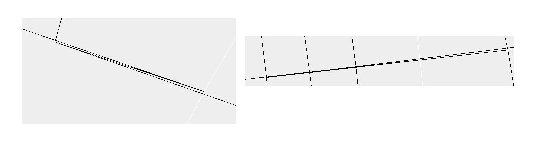
\includegraphics[scale=1.0]{routefailure.eps}
   \caption{Example Failures in Street Map}
   \label{fig:routefailure}
   \end{center}
\end{figure}
at two places. We corrected the source file ``streets.data`` delivered by \bmodb{}
at this two routes and restarted the building of the databases and our experiments
from the scratch. After all results from the network queries corresponded to the
results of the \bmodb{} results we figured out the fastest versions of the
executable \secondo{} network queries and started them several times to measure
the run times analogues to the run times of the \bmodb{} benchmark queries. The
results of the run time measurement are shown in \ref{sec:results}.
\subsection{Translation of BerlinMOD into Network Data Model}
\label{sec:Translation}
The construction of the central \dt{network} object from the $streets$ value
of the \bmodb{} is described in section \ref{sec:createNetwork}. We used this
\dt{network} object to transfer the spatial and spatio-temporal data objects into
the network data model representation (see \ref{sec:translateSTdata}). We build
several indexes on this spatial-temporal network constrained data (see
\ref{sec:createIndex}) to support faster query execution. We conclude the subsection
with a description of our executable \secondo{} network queries for the \bmodb{}
in section \ref{sec:queries}.

On our website \cite{berlinmodweb} we provide different \secondo{} scripts. One
for the network data creation, the translation of the \bmodb{} data sets into
network data representation, and the index generation. And two scripts containing
the network query sets for the object and the trip based approach of the \bmodb{}.
\subsubsection{Create Network Object}
\label{sec:createNetwork}
For the creation of the \dt{network} object $net$ representing the street map of
Berlin we extract the routes data from the $streets$ relation of the \bmodb{}
data set. The extracted routes data $r$ is used to compute the crossings of the
routes of Berlin $j$. In this step the connectivity code for each crossing is
set to the maximum value because the data source lacks on information about the
connectivity of the crossings.
We use $r$ and $j$ as input relations for the creation of our \dt{network}
object $net$ representing the streets of Berlin in the network data model.

The network creation algorithm first copies all tuples of $r$ to the
$routes relation$ of $net$ and creates the B-Tree index of the route
identifiers and the R-Tree index of the route curves of the $routes relation$ of
$net$. Then all tuples of $j$ are copied to the $junctions relation$
of $net$ and the $tuple identifiers$ for the both routes connected
by this junction are added to the junctions entry in the $junctions relation$.
After that we build two B-Trees indexes over the route identifiers of the first
respectively second route in the $junctions relation$. Next for every route of the
$routes relation$ all junctions on this route are taken to compute the up and
down sections for each of this junctions on the route. The up and down
sections are inserted into the $sections relation$ of $net$ and the
$tuple identifiers$ of the sections are added to the entry of the according
junction in the $junctions relation$. After that the B-Tree index for the
route identifiers in the $sections relation$ is created and the adjacency
lists of $net$ are filled with the adjacent section pairs defined by the
$junctions relation$.

If $|r|$ is the number of routes and $|j|$ is the number of junctions.
The algorithm needs O($|r| \log |r|$) time to copy $r$ to the
$routes relation$ of $net$ and create the indexes of the
$routes relation$. The creation of the $junctions relation$ and the build
of the B-Trees indexes takes O($|j| \log |j|$) time.
O($|r||j|$) time is needed to fill the $sections relation$ and
O($|j|$) time to fill the $adjacency lists$ of $net$. Alltogether
the complete algorithm needs:
O($|r| \log |r|+|j| \log |j| + |r||j|$)
 time to create the $net$ from the two input relations $r$ and $j$.
\subsubsection{Translate Spatial and Spatio-Temporal Data}
\label{sec:translateSTdata}
In this section we describe the translation of the spatial and spatio-temporal
data types of the \bmodb{} data set into spatio-temporal network objects. The
translation is done relative to the \dt{network} object $net$ (see  \ref{sec:createNetwork}).
The input for all algorithms is a spatial respectively
spatio-temporal \bmodb{} data object and the \dt{network} object $net$.
If a input data object is not constrained by $net$ the translation result is
undefined for all network translation algorithms.

We start the explanation of our translation algorithms with the \op{point2gpoint}
operation, because this operation is used by the other translation algorithms.
The algorithm translates a \dt{point} value $p$ into a corresponding
\dt{gpoint} value $gp$. It uses the R-Tree index of the $net$
$routes relation$ to select the route closest to $p$ and computes the
position of $p$ on this route. The $side$ value of $gp$ is always set
to $none$. Because the \bmodb{} does not differntiate between the sides of a
road. If $r$ is the number of routes in the $net$ $routes relation$
and $k$ is the number of possible candidate routes the worst case complexity
of the algorithm is O($k + \log r$).

This should be all to translate the \dt{point} values of the $QueryPoints$
relation of the \bmodb{} into network query positions. But there is a problem with
the network data model representation of junctions. In the network data model
contrary to the data model of freely moving in space junctions have more than one
\dt{gpoint} representation, because they are related to two or more routes. Hence
if a junction position is given related to route $a$ we won't detect the
junction as passed if a \dt{mgpoint} object passes the junction on route $b$
in all cases, because the definition of \op{passes} in the network data model is
slightly different from the \op{passes} operation in the \bmodb{} data model.
Unfortunately all query points of the \bmodb{} are junctions. As work around we
added a operator \op{polygpoints}, which returns for every input \dt{gpoint}
value $gp$ a stream of \dt{gpoint} values. If $gp$ represents a junction
we return all \dt{gpoint} values representing the same junction in $net$,
otherwise we return only $gp$ in the stream. So we got 221 query \dt{gpoint}
values in $QueryPointsNet$ for the 100 query \dt{point} values in
$QueryPoints$ and 22 \dt{gpoint} values in $QueryPoints1Net$ for the
10 \dt{point} values of $QueryPoints1$ of the \bmodb{}. This means we have
always to compute the results for the doubled number of query points in our network
data model than in the data model of free movement in space.

The second operation \op{mpoint2mgpoint} translates a \dt{mpoint} value $s$
into a \dt{mgpoint} value $t$. The main idea of the algorithm is to use the
continuous movement of $s$ to reduce computation time. We initialize the
algorithm by reading the first unit of $s$ and use the \op{point2gpoint}
operation to find a route in the network containing the $start$ and
the $end point$ of this unit. We initialize the first unit of $t$ with
the computed network values. Then we read the next unit of $s$ and try to find
the $end point$ of the new unit on the same route the last unit of $s$ was
found. If the $end point$ is found on this route we check the direction and
speed of the unit. If they are equal to the last unit we extend the actual unit
of $t$ to enclose the value of the actual unit of $s$. If the speed or
the moving direction changes we write the actual unit to $t$ and initialize
a new unit for $t$ with the network values of the actual unit from $s$.
If the $end point$ can't be found on the same route than the last unit from
$s$ we write the actual unit of $t$ and start a search on the route curves
of the adjacent sections to find the route curve that contains the $start$
and the $end point$ of the actual unit of $s$. We initialize a new unit
for $t$ with the estimated network values for the actual unit of $s$ and
continue with the next unit of $s$. At least we add the actual network unit
to $t$.

The time complexity to find the start values for the first unit is O(\op{point2gpoint}).
For the next $m$ units of $s$ the time complexity is O(1) if $s$ don't change the
route. And O($a$) if the end point is on another route and $a$ is the maximum
number of adjacent sections. So we get a worst case time complexity of
O(O(\op{point2gpoint}) + $ma$) for the translation of a \dt{mpoint} $s$ into a
\dt{mgpoint} $t$.

The translation of the \dt{region} values in the $QueryRegions$ relation of the
\bmodb{} into \dt{gline} values of our network data model is done in several steps.
First of all we build a single big \dt{line} object from all our network streets.
Then we compute for each \dt{region} of the $QueryRegions$ the intersection with
this big \dt{line} object. At least we translate the resulting \dt{line} objects
of the intersection, each representing one \dt{region} of the $QueryRegions$
relation, into sorted \dt{gline} values using the \op{line2gline} operation.
The algorithm of the \op{line2gline} operation takes each half segment of a
\dt{line} value and computes a corresponding network route interval by
searching a common route curve for the $start$ and the $end point$ of the
half segment using the \op{point2gpoint} operation. The computed
route intervals are sorted, merged and compressed before the resulting
\dt{gline} value is returned. If the number of half segments of a \dt{line}
value is $h$ and the number of resulting compressed route intervals is $r$
we get a time complexity of O($h$O(\op{point2gpoint})$+ h \log r + r$) for the
whole algorithm. Whereby the summand $h \log r + r$ is caused by the compressing
and sorting of the resulting \dt{gline} but as mentioned before
in \ref{sec:sortedgline} we think this time is well invested.
\subsubsection{Create Indexes on Network Data Model}
\label{sec:createIndex}
After translating all the \bmodb{} data sources we are able to create indexes on
our network data representation of the \bmodb{} data. First we create B-Trees
for the $licences$ and $moid$ attributes of the relations $dataSNcar$, and $dataMNtrip$.
This indexes are similar to the indexes created in the \bmodb{} for $dataSCcar$,
and $dataMCtrip$, because the relations $dataSNcar$ and $dataMNtrip$ contain
the network data model representation of the $dataScar$ and $dataMtrip$ relation
of the \bmodb{}. Then we create R-Tree indexes over the spatio-temporal bounding
boxes of the \dt{mgpoint} attributes in the $dataMNtrip$ and the $dataSNcar$ relation.
At least we create some specialized network indexes indicating network positions
and network-temporal positions of moving objects. Therefore we introduce two and
three dimensional $netboxes$. A $netbox$ is a degenerated two or three
dimensional rectangle. The coordinates of the rectangle are defined to be
$x_1 = x_2 = route identifier$ as \dt{real} value (The equality of $x_1$ and
$x_2$ makes the degeneration.), $y_1 = \min (star position, end position)$,
$y_2 = \max (start position, end position)$,
and, in the three dimensional case, $z_1 = starttime$ as \dt{real} value and
$z_2 = endtime$} as \dt{real} value.  For every unit of each \dt{mgpoint} we
build a three dimensional $netbox$ and for every $route interval$ of every
\dt{mgpoint}s trajectory a two dimensional $netbox$. This $netboxes$ are used to
create R-Trees indexing the network and network-temporal positions of the \dt{mgpoint}s
in the network data model representation of the \bmodb{}.
\subsubsection{Translate Benchmark Queries}
\label{sec:queries}
We developed executable \secondo{} queries for each of the 17 BerlinMOD/R queries
for the object based approach (OBA) and the trip based approach (TBA) using our
network indexes to support faster query execution. We had to do this manually
because the \secondo{} optimizer is not able to optimize SQL-queries on network
data model objects yet. In our experiments we tried many different query
formulations for each query to get optimal queries delivering the correct result
in a minimum of time. The limited space does not allow us to show all our
executable \secondo{} network queries in detail. As mentioned before the complete
\secondo{} network scripts can be taken from our website. In the following we
describe only the algorithms of a few queries in detail.

Every time we need a licence in the result or have a query licence number we need
a additional step in the TBA. Because we have to join the tables
$dataMNtrip$ and $dataMNcar$ using the $moid$ attribute and the corresponding
B-Tree indexes. We will not repeat this step at every single
query description.

Query 1 and 2 work only on standard attributes. They are formulated analogous to
the original queries of the \bmodb{} only the relation names and the used B-Trees
are changed to match the network data model.

Query 3 uses the licence B-Tree to select the ten cars with licences from
$QueryLicences1$ from $dataSNcar$ then the positions of this cars are computed
for each of the ten time instants from $QueryInstants1$.

In Query 4 we produce a $netbox$ for each of the $QueryPointsNet$ and use our
specialized netbox R-Tree of the \dt{mgpoint} $route intervals$ to select
the passing vehicles.

In the queries 5, 6, and 10 a retransmission of network objects into spatial
respectively spatio-temporal objects of the \bmodb{} data model is done. This is
caused by the fact that
the \bmodb{} deals with Euclidean Distances. Euclidean Distances are not very useful
in network environments because all objects are restricted to use network paths.
Therefore in networks normally the Network Distance is computed. To make the results
comparable we retransmit the intermediate results of our network data model into
spatial and spatio-temporal data types and use the existing spatial and
spatio-temporal Euclidean Distance Functions of the \bmodb{} data model for the
distance computation in the queries 5, 6, and 10.

Query 5 selects the cars with $licences$ from $QueryLicence1$ respectively
$QueryLicences2$  using the B-Tree over the $Licence$ attribute of $dataSNcar$
and creates a \dt{line} value  from the list of $route intervals$ passed by
every car. Then the Euclidean Distance between this \dt{line} values is computed
for each pair of licences one from $QueryLicences1$ and one  from $QueryLicences2$.
In the TBA we need a aggregation step building the union of the several
\dt{mgpoint} belonging to each candidate car. This is done with the $route intervals$
returned as trajectory of the \dt{mgpoint} values because it takes much less
time to build the union of the $route intervals$ than of the half segments
in the \dt{line} values representing the same network part.

Query 6 uses the \op{filter} operation to select the ''trucks`` from $dataSNcar$
(respectively $dataMcar$ in TBA) relation. Then the spatio-temporal bounding box of
each trip is computed and the spatial dimensions of this box are extended by 5m in
every spatial direction. After that the \dt{mgpoint} values are retranslated into
\dt{mpoint} values. In a second step each result of the first step is joined with
all other results of the first step if the extended bounding boxes intersect, the
licences are different and the \dt{mpoint} values have sometimes a distance lower
than 10m. The licence pairs of trucks fullfilling this predicate are returned. In
the TBA there might be duplicate licence pairs which we have to remove before we
return the result.

The first part of the first step of query 7 is almost equal to the selection of cars
passing a query point in query 4. The intermediate result is filtered to remove all
``not passenger'' cars and for every remaining trip the time the trip reaches first
the query position is computed for every query position and every candidate trip. In
a second step the resulting time instants are grouped by the $id$ of the query
positions and the minimum time stamp of each group is computed. This minimum time
stamp is for every query position the first time it was reached by a car. In the
third and last step the licences of the cars reaching the query positions at this
first time instant are computed by a join of the results of the first two steps by
query position id and the equality of the time stamps.

In query 8 we just select the candidate cars with the licence B-Tree and compute for
every car the length of the trip at the query periods in the OBA. In the TBA we have
to aggregate over all the distances driven in the single trips by a car within a
query period.

For query 9 we compute the length of every trip in every query period, and select the
maximum driven distance for every period. In the TBA again we have to do a
aggregation of the distances driven from the same car in the same period.

For query 10 in OBA we first retranslate every \dt{mgpoint} value of $dataSNCar$ into
a \dt{mpoint} value and extend the spatial bounding box of each of this
trips by 1.5 m in every direction. Second we select the ten candidate trips given by
$QueryLicences1$, retranslate them and extend their spatial bounding boxes. Than we
join all trips from the first and the second step where the
extended bounding boxes intersect. We filter the pairs that have different licences
and are sometimes nearer than 3m. For this pairs we compute the position of the
\dt{mgpoint} at the times the distance between the both \dt{mpoint} has been smaller
than 3 m. We return the licence pairs and the positions when they have been closer
than 3 m to each other. In TBA we select the trips given by $QueryLicences1$ from
$dataMNtrip$ retranslate them into \dt{mpoint} values. Then we use the
spatio-temporal index of $dataMNtrip$ to select for each of the ten cars the cars
of $dataMNtrip$ which bounding boxes intersect the extended spatio-temporal bounding
boxes of the first selected candidate trips. For every pair of candidate trips we
retranslate the second trip into free movement and use the Euclidean Distance
function for \dt{mpoint} values to determine the deftimes when the both \dt{mgpoint}
had a distance lower than 3m. At least we restrict the trips on this times and
aggregate the resulting trips into one single trip for each licence pair.

In our experiments we tried out several indexes to support faster query execution of
especially of query 10 including the MON-Tree \cite{MONTree}. But at the end this
simple form shows the best complete run time performance of all indexes.

In query 11 we build a network-temporal query box from the product of $QueryInstant$
and $QueryPoints1Net$ relation. And use the network-temporal index on $dataSNcar$
(respectively $dataMNtrip$) to select the resulting trips.

The first step of query 12 is identical with query 11. In a second step a product of
the result of the first step with itself is computed and checked for vehicles which
have been at the same query point at the same query time instant.

Query 13 first computes uses the trajectory value of the \dt{mgpoint} to select the
trips passing a given region. Restricts the trips to the times they pass the region
and tests the resulting trips for their existenz in a given time interval. In TBA
possible duplicate licence pairs have to be removed and the resulting $moids$ must
be mapped to the licences of the cars to generate the result.

Query 14 and 15 build sets of three dimensional network boxes of the query parameters
and use the three dimensional network box tree to select the candidate trips. The
resulting candidate trips are filtered to be sure they realy fullfill the query
constraints.

Query 16 selects the candidate trips using the licence B-Tree, filters them to be \op{present} within the query periods and restricts them to the times of the query periods. The restricted trips are filtered with the \op{passes} operation and restricted
to the times they were inside the query region. This is done one time
for $QueryLicences1$ and one time for $QueryLicences2$. The both results are joined
to get the trips of different cars which where at the same period in the same region
without meeting each other there and then in a third step. Again in the TBA we have
to do a additional selection from trips with the $moids$ belonging to the cars
selected before by the licences and to remove duplicates of licence pairs in the
same period.

Query 17 again uses the methods from query 4 to find the trips passing a given query
point. The passing cars are grouped by the passed query points and the number of
cars per query point is computed. In a second step the point with the maximum number
of hits is selected and his id and the number of passing cars is returned. In the
TBA we have to remove the duplicate cars from the result before computing the hits.
\subsection{Benchmark Results}
\label{sec:results}
We made several runs for each data amount and each query to get correct average execution times for each query in both data models. Table \ref{tab:dbstatistic} compares the creation times, the number of units and the storage space of the both data models at the different $scalefactors$.
\begin{table}[H]
\begin{center}
\begin{scriptsize}
\begin{tabularx}{1.0\textwidth}{|X|c|c|c|c|c|c|}
\hline
&\multicolumn{2}{c|}{\textbf{Scalefactor 0.05}}&\multicolumn{2}{c|}{\textbf{Scalefactor 0.2}}&\multicolumn{2}{c|}{\textbf{Scalefactor 1.0}}\\
\hline
No. of Cars&\multicolumn{2}{c|}{447}&\multicolumn{2}{c|}{894}&\multicolumn{2}{c|}{2000}\\
\hline
No. of Days&\multicolumn{2}{c|}{6}&\multicolumn{2}{c|}{13}&\multicolumn{2}{c|}{28}\\
\hline
Data Generation&\multicolumn{2}{c|}{164.761s}&\multicolumn{2}{c|}{587.299s}&\multicolumn{2}{c|}{3177.46s}\\
\hline
&BMODB&Network&BMODB&Network&BMODB&Network\\
\hline
Data Translation
and Index Build&301.72s&535.65s&1,362.72s&2,190.45s&7419.130&11,144.13s\\
\hline
No. of Units&2,646,026&1,260,888&11,296,682&5,346,971&52,140,685&24,697,709\\
\hline
Storage Space&2.26 GB&0.86 GB&9.51 GB&3.69 GB&45,76 GB&17.28 DB\\
incl. Data&0.79 GB&0.44 GB&3.35 GB&1.83 GB&15.47 GB& 8.40 GB\\
incl. Indexes&1.48 GB&0.42 GB&6.16 GB&1.86 GB&30.30 GB&8.89 GB\\
\hline
\end{tabularx}
\end{scriptsize}
\caption{Database Statistics}
\end{center}
\label{tab:dbstatistic}
\end{table}
As you can see the network data model needs less than 40\% of the storage space from
the \bmodb{} data model. The main cause is that the same trip is represented
by less than 50\% of the units in the network data model compared to the data
model of free movement in the two dimensional space. And that although in towns
cars often change the speed or the used street. We expect this effect to be much
higher if the cars go for long trips between different towns especially if they
use highways.

The long creation time for the network data model representation is
caused by the expensive mapping of spatial and spatio-temporal positions into
network positions. The Indexes are build faster in the network representation
because they are much smaller than in the \bmodb{} data representation.

Figure \ref{fig:compruntimes} shows the run times for all queries in both data
models in seconds. And the grafic compares the total runtimes of the query sets
in the different data representations.
\begin{figure}[h]
  \begin{minipage}{0.5\linewidth}
    \begin{tiny}
      \begin{tabular}{|c|r|r|r|r|}
        \hline
        &\multicolumn{4}{c|}{\textbf{Scalefactor 0.05}}\\
        \hline
        &\multicolumn{2}{c|}{\textbf{BMODB}}&\multicolumn{2}{c|}{\textbf{Network}}\\
        \hline
        \textbf{Query}&\textbf{OBA}&\textbf{TBA}&\textbf{OBA}&\textbf{TBA}\\
        \hline
        \textbf{1}&0.086&0.100&0.090&0.113\\
        \hline
        \textbf{2}&0.003&0.003&0.003&0.002\\
        \hline
        \textbf{3}&0.346&0.345&0.112&0.568\\
        \hline
        \textbf{4}&9.105&15.403&0.142&1.303\\
        \hline
        \textbf{5}&1.076&1.623&0.927&1.377\\
        \hline
        \textbf{6}&16.781&14.934&5.004&4.483\\
        \hline
        \textbf{7}&2.996&3.007&1.221&6.790\\
        \hline
        \textbf{8}&0.346&0.424&0.225&0.213\\
        \hline
        \textbf{9}&99.375&193.929&22.935&24.349\\
        \hline
        \textbf{10}&139.795&36.636&81.770&84.298\\
        \hline
        \textbf{11}&0.143&0.111&0.158&0.898\\
        \hline
        \textbf{12}&0.297&0.133&0.228&0.202\\
        \hline
        \textbf{13}&11.284&7.341&1.159&1.336\\
        \hline
        \textbf{14}&0.525&0.727&0.793&3.734\\
        \hline
        \textbf{15}&1.201&0.802&0.625&0.543\\
        \hline
        \textbf{16}&43.567&5.346&0.680&1.579\\
        \hline
        \textbf{17}&1.084&0.935&0.234&0.337\\
        \hline
        \textbf{Total}&328.009&281.797&116.305&132.127\\
        \hline
      \end{tabular}
    \end{tiny}
  \end{minipage} \hfill
\begin{minipage}{0.5\linewidth}
    \begin{tiny}
      \begin{tabular}{|c|r|r|r|r|}
        \hline
        &\multicolumn{4}{c|}{\textbf{Scalefactor 1.0}}\\
        \hline
        &\multicolumn{2}{c|}{\textbf{BMODB}}&\multicolumn{2}{c|}{\textbf{Network}}\\
        \hline
        \textbf{Query}&\textbf{OBA}&\textbf{TBA}&\textbf{OBA}&\textbf{TBA}\\
        \hline
        \textbf{1}&0.226&0.166&0.185&0.215\\
        \hline
        \textbf{2}&0.005&0.004&0.019&0.004\\
        \hline
        \textbf{3}&0.745&0.845&0.845&1.323\\
        \hline
        \textbf{4}&149.167&427.583&1.145&31.879\\
        \hline
         \textbf{5}&3.029&5.821&4.781&5.277\\
        \hline
        \textbf{6}&1463.214&5110.613&381.622&263.371\\
        \hline
        \textbf{7}&84.660&50.575&124.602&169.848\\
        \hline
        \textbf{8}&0.890&0.557&0.258&0.303\\
        \hline
        \textbf{9}&830.253&3153.720&120.470&156.693\\
        \hline
        \textbf{10}&4414.632&2015.096&2786.578&1791.941\\
        \hline
        \textbf{11}&0.656&0.914&6.030&7.738\\
        \hline
        \textbf{12}&36.210&0.213&0.274&0.267\\
        \hline
        \textbf{13}&119.685&94.366&29.126&36.086\\
        \hline
        \textbf{14}&10.912&3.915&36.041&38.552\\
        \hline
        \textbf{15}&30.874&18.711&10.317&7.989\\
        \hline
        \textbf{16}&35.490&8.655&0.584&1.969\\
        \hline
        \textbf{17}&82.242&343.826&0.550&8.026\\
        \hline
        \textbf{Total}&7262.888&11235.581&3503.429&2521.481\\
        \hline
      \end{tabular}
    \end{tiny}
  \end{minipage}\hfill
  \begin{minipage}{0.5\linewidth}
    \begin{tiny}
      \begin{tabular}{|c|r|r|r|r|}
        \hline
        &\multicolumn{4}{c|}{\textbf{Scalefactor 0.2}}\\
        \hline
        &\multicolumn{2}{c|}{\textbf{BMODB}}&\multicolumn{2}{c|}{\textbf{Network}}\\
        \hline
        \textbf{Query}&\textbf{OBA}&\textbf{TBA}&\textbf{OBA}&\textbf{TBA}\\
        \hline
        \textbf{1}&0.146&0.123&0.082&0.092\\
        \hline
        \textbf{2}&0.003&0.003&0.004&0.003\\
        \hline
        \textbf{3}&0.456&0.523&0.134&0.834\\
        \hline
        \textbf{4}&32.832&80.881&0.217&7.504\\
        \hline
        \textbf{5}&1.539&2.824&1.768&2.251\\
        \hline
        \textbf{6}&70.266&120.294&20.605&14.884\\
        \hline
        \textbf{7}&14.479&10.423&10.107&35.036\\
        \hline
        \textbf{8}&0.435&0.446&0.202&0.225\\
        \hline
        \textbf{9}&237.581&485.998&41.579&50.853\\
        \hline
        \textbf{10}&605.718&139.565&378.248&309.345\\
        \hline
        \textbf{11}&0.233&0.149&0.178&3.017\\
        \hline
        \textbf{12}&4.332&0.160&0.269&0.260\\
        \hline
        \textbf{13}&1.30.173&13.791&5.737&5.248\\
        \hline
        \textbf{14}&1.115&1.166&1.469&9.286\\
        \hline
        \textbf{15}&8.824&4.286&2.644&2.084\\
        \hline
        \textbf{16}&29.389&5.500&0.376&0.847\\
        \hline
        \textbf{17}&8.453&4.169&0.306&0.923\\
        \hline
        \textbf{Total}&1045.974&870.300&463,926&442.691\\
        \hline
      \end{tabular}
    \end{tiny}
  \end{minipage}\hfill
  \begin{minipage}{0.5\textwidth}
      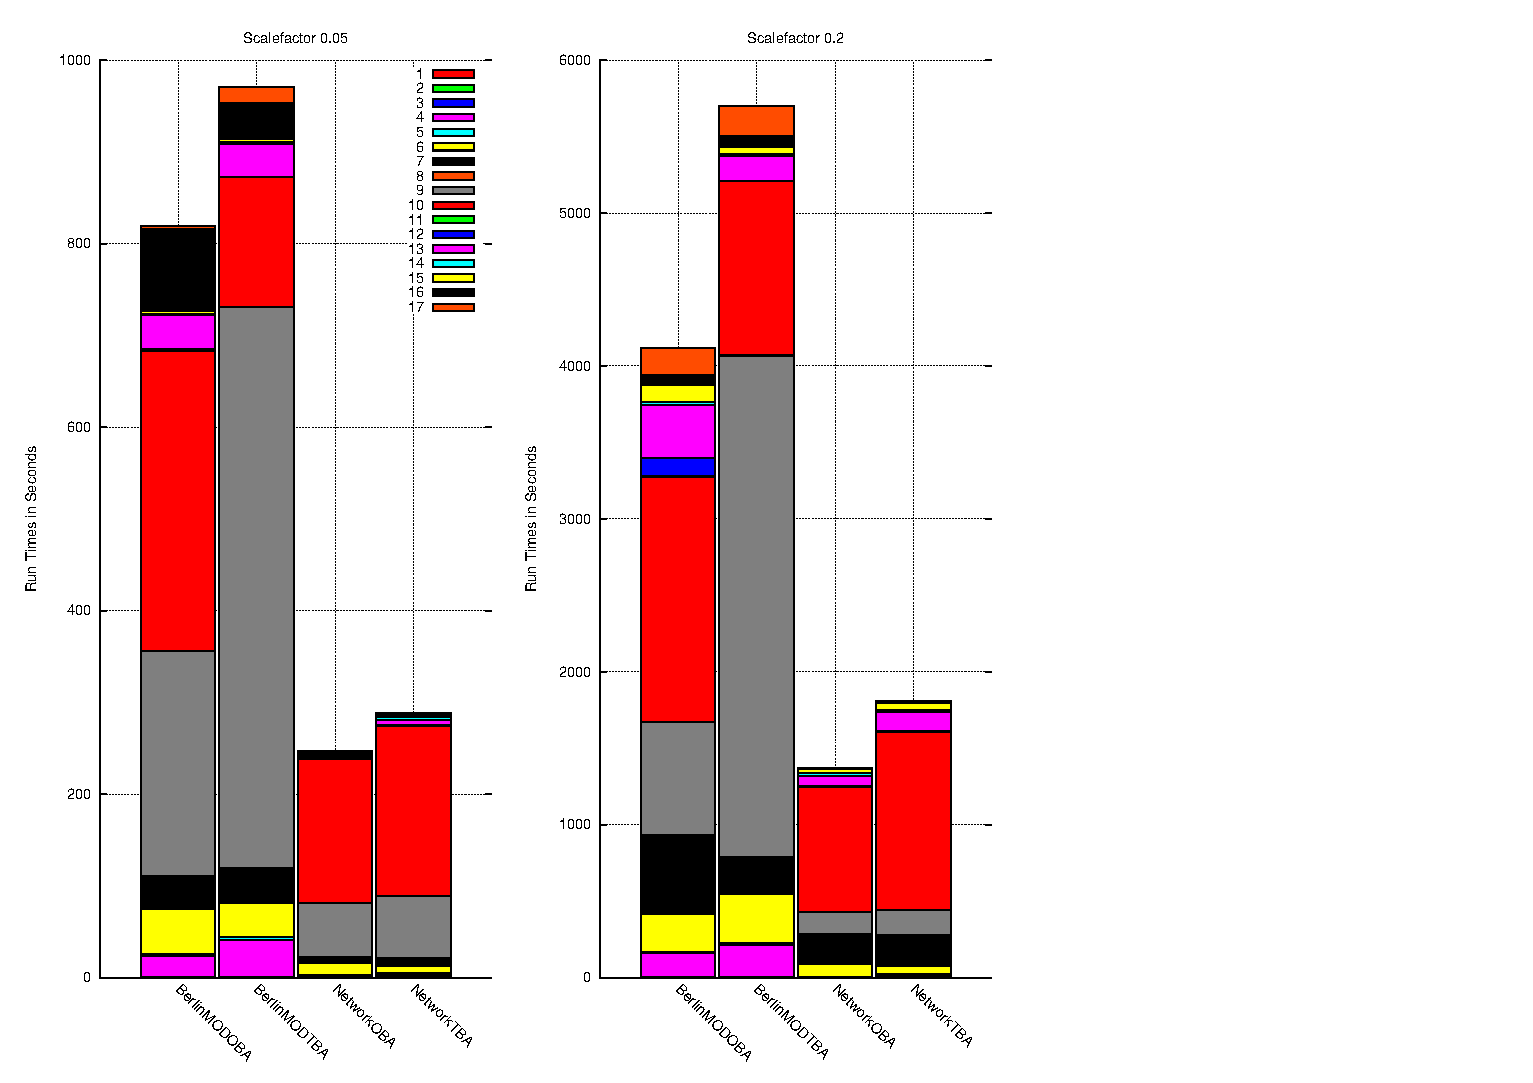
\includegraphics[width=0.8\linewidth]{compruntimesall.eps}
  \end{minipage}
 \caption{Compare Run Times}
 \label{fig:compruntimes}
\end{figure}
As you can see the total run time of all queries in the network data model is less than 50\% of the total run time in the data model of free movement in the space at each scalefactor.

%\begin{figure}[H]
%\begin{center}
%   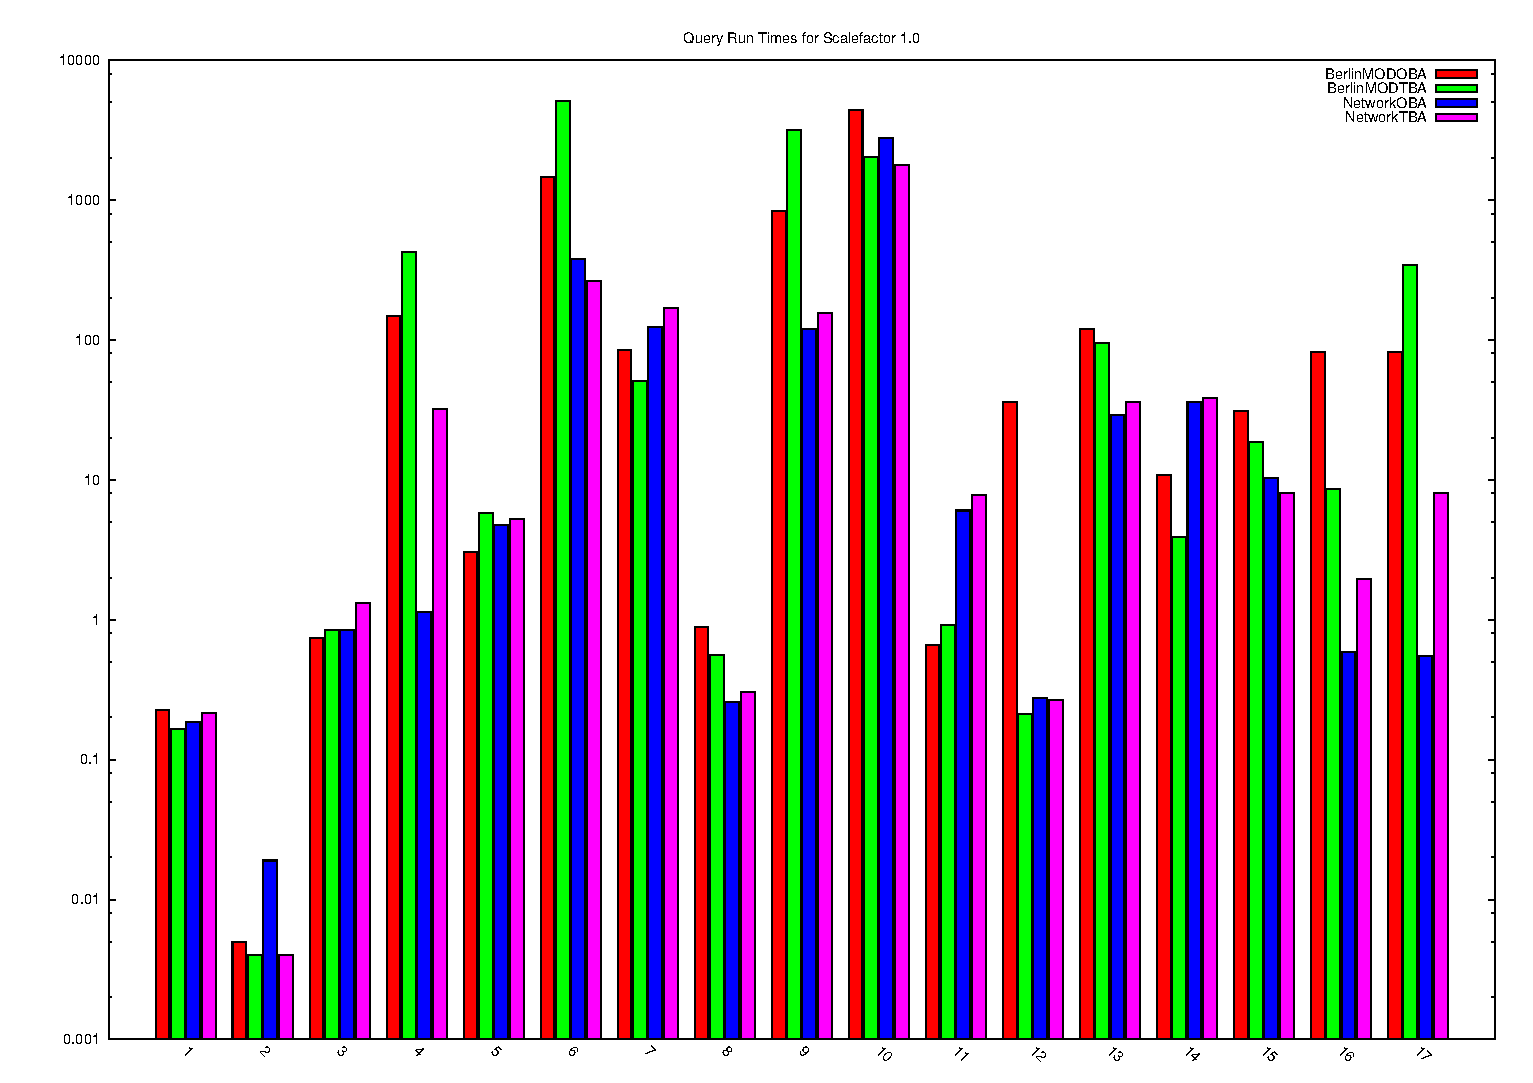
\includegraphics[width=1.0\textwidth]{compqueryruntimes.eps}
%   \caption{Compared Run Times for Each Query at Scalefactor 1.0}
%   \label{fig:compqueryruntimesall}
%\end{center}
%\end{figure}

\section{New BerlinMOD Queries}
\label{sec:newqueries}
\section{Summary and Future Work}
\label{sec:summary}
Our experiments show that the network data model of moving in free space
 outperforms the \bmodb{} data model in the total query run time and in the most
single cases. The good results of the network data model encouraged us to extend
the \bmodb{} with a set of queries that enables us to compare the capabilities of
 different spatio-temporal network data models with respect to the specialized
 challenges of this data models.

\bibliography{BerlinMODAndNetworkDataModel}{}
\bibliographystyle{plain}
\end{document}
